\section{Additional Tools}
\subsection{Splitting a link}
Links can be split in two separate parts and it is possible to change location
of both of its parts after selecting it with the \emph{Select tool}. Right
click on the link and than left click on the \emph{Split label} in the pop-up
menu to split the link in two halves. Separated link parts can be merged back
with the \emph{Merge} option from the link menu. This feature is shown in
Figure \ref{fig:split_link}.

\begin{figure}[H]
\centering
\vspace{10pt}
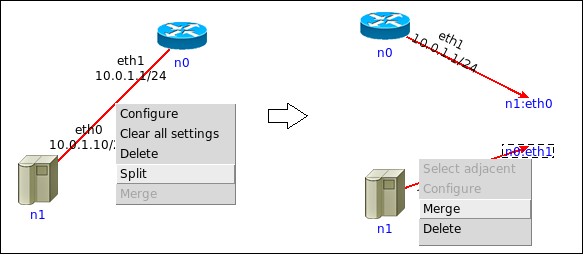
\includegraphics[width=0.7\textwidth]{./images/split_link.png}
\caption{\emph{Split link}}
\label{fig:split_link}
\end{figure}

\subsection{Generating a network topology}
\label{sec:GeneratingNetworkTopology}
\emph{TopoGen} menu from the menubar enables easier and faster generation of
network topologies (Figure \ref{fig:topogen_menu_star}). This function can be
used to generate following topologies: \emph{Chain, Star, Cycle, Wheel, Cube,
Clique, Bipartite} or \emph{Random}. 

\begin{figure}[H]
\centering
\vspace{10pt}
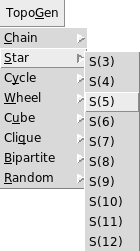
\includegraphics[width=0.18\textwidth]{./images/topogen_menu_star.png}
\caption{\emph{TopoGen menu}}
\label{fig:topogen_menu_star}
\end{figure}

Some examples can be seen in Figure \ref{fig:star}, Figure \ref{fig:bipartite}
and Figure \ref{fig:wheel}. In order to generate a topology first select the
network layer nodes (router, host or PC) from the toolbox and then the desired
topology type e.g. bipartite graph K(2,3) (see Figure \ref{fig:bipartite}).

\begin{figure}[H]
\centering
\vspace{10pt}
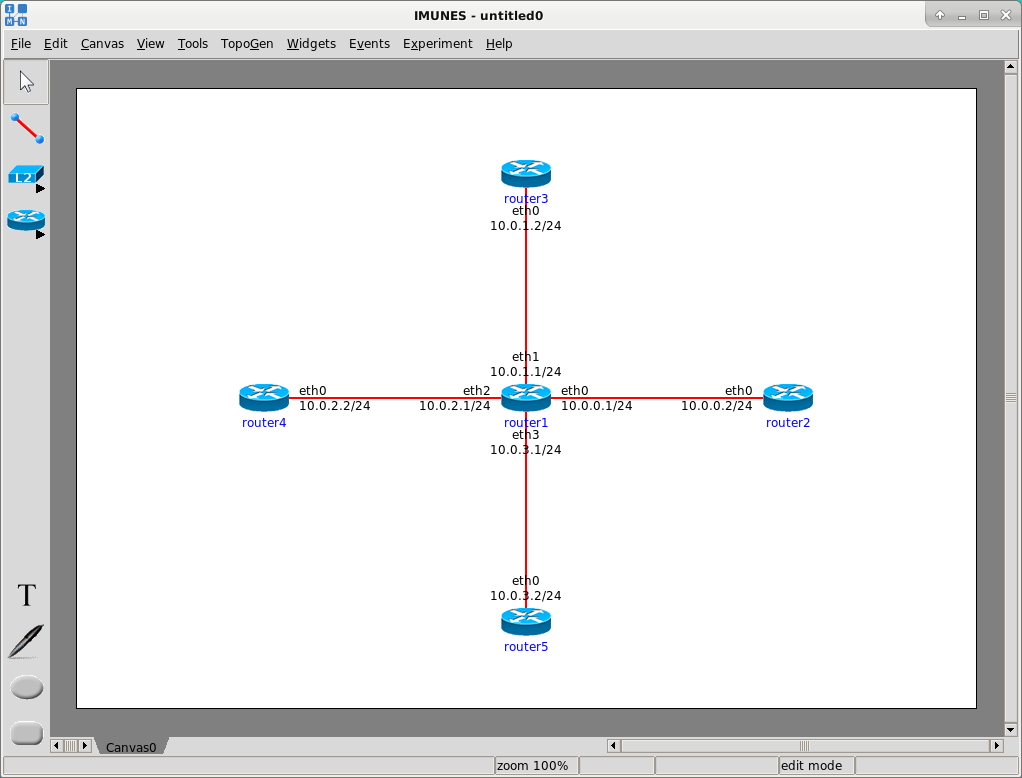
\includegraphics[width=\textwidth]{./images/star.png}
\caption{\emph{Star topology}}
\label{fig:star}
\end{figure}

\begin{figure}[H]
\centering
% \vspace{10pt}
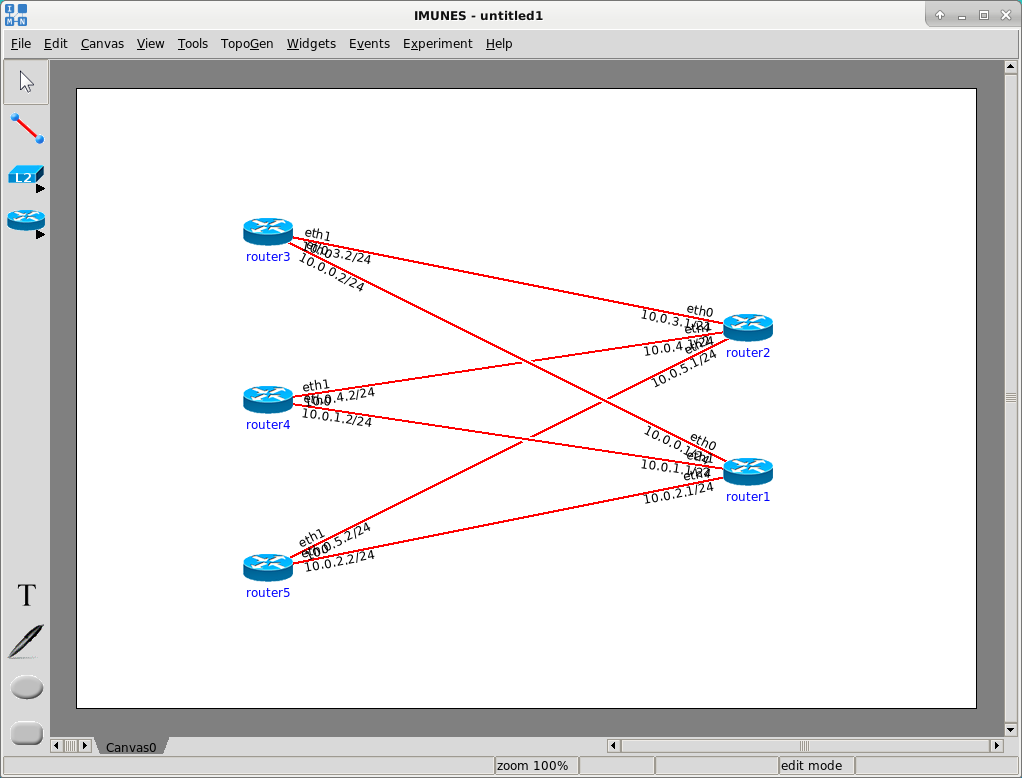
\includegraphics[width=\textwidth]{./images/bipartite.png}
\caption{\emph{Bipartite topology}}
\label{fig:bipartite}
\end{figure}

\begin{figure}[H]
\centering
% \vspace{10pt}
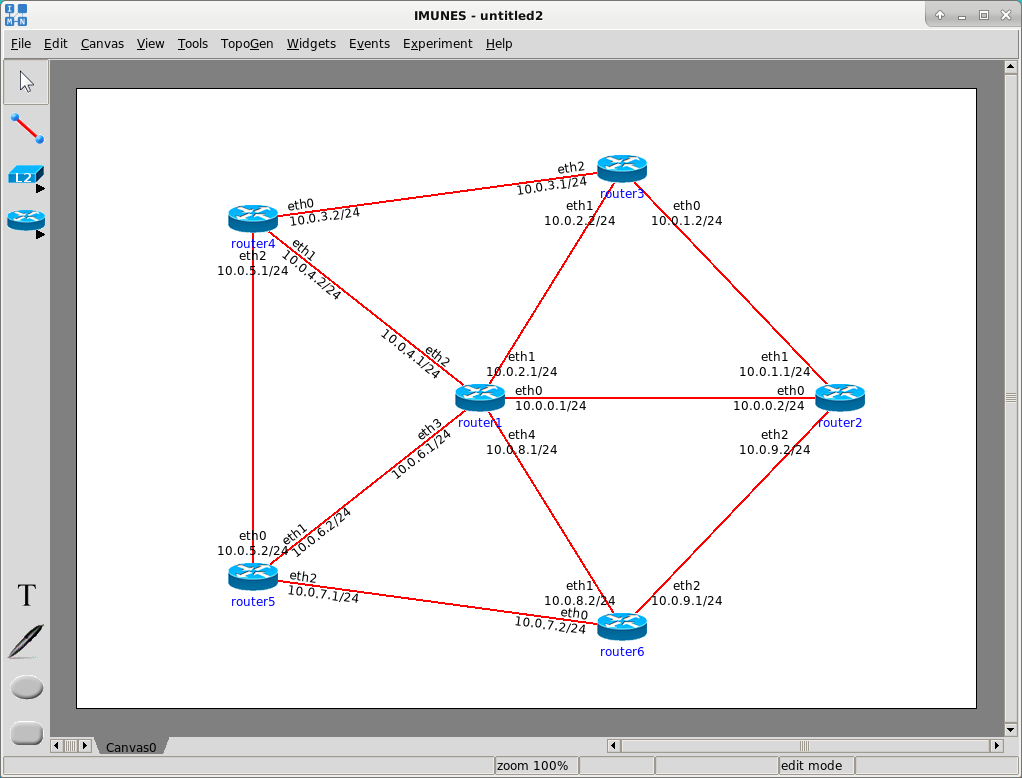
\includegraphics[width=\textwidth]{./images/wheel.png}
\caption{\emph{Wheel topology}}
\label{fig:wheel}
\end{figure}  

In case of \emph{random} topology an additional information is needed, so
beside the number of the nodes it is also necessary to specify the number of
links. The nodes in the random topology will be randomly connected with the
number of links specified before. An example of generating a \emph{random}
topology: 
  \begin{enumerate}
  \item Select the router tool from the toolbox.
  \item Choose the random topology: \emph{TopoGen $\to$ Random}
  \item Choose the desired number of nodes and links e.g. n = 6; m = 5, where n
is the number of nodes and  m  the number of links in the generated network
topology (\emph{Random $\to$ R(6,m) $\to$ R(6,5)}). 
 \end{enumerate}
 The result is shown in Figure \ref{fig:random}. 
 
\begin{figure}[H]
\centering
\vspace{10pt}
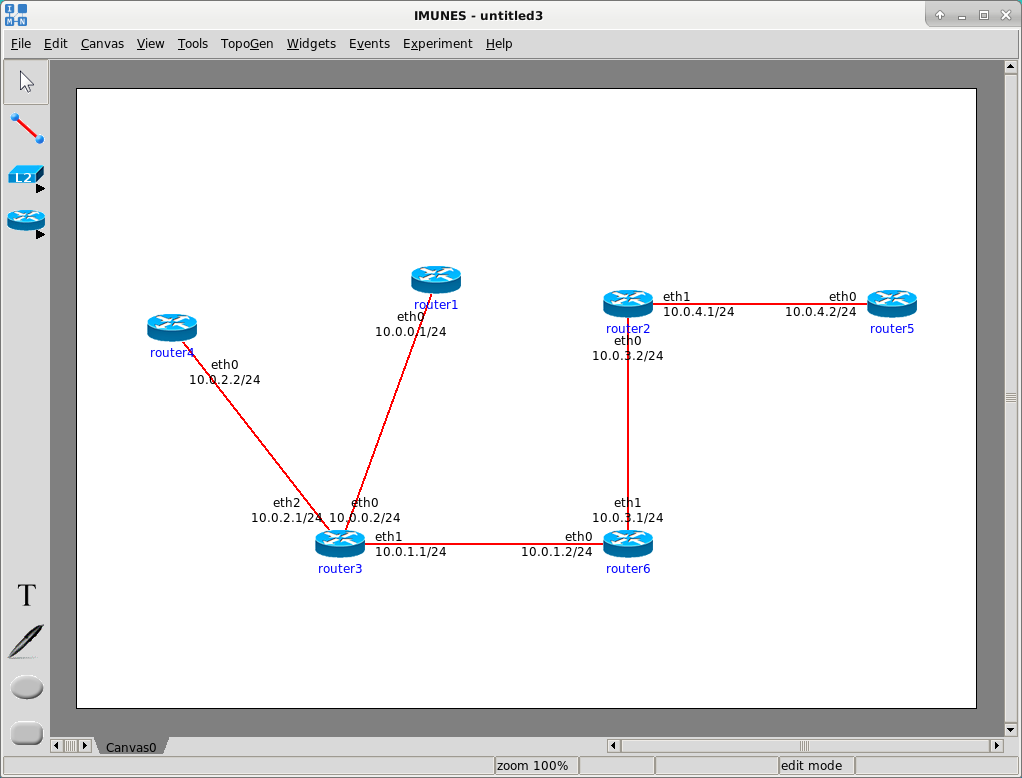
\includegraphics[width=\textwidth]{./images/random.png}
\caption{\emph{Random topology}}
\label{fig:random}
\end{figure} 
 
Using the \emph{TopoGen} tool you can generate topologies containing one type
of node (router, host or PC). In that case, new nodes of the same type are
created and placed on the canvas. Another option is to add new nodes to canvas
and then connect them using the topology generator:
\begin{enumerate}
  \item Add nodes to the canvas (don't have to be same type). 
  \item Select nodes that should be included in the new topology
  \item Right click on one of the selected nodes and choose the option
\emph{Create Link to} from the menu. Choose the option \emph{Selected} and
select one of the offered topologies (\emph{Chain, Star, Cycle, Clique} or
\emph{Random}). An example is shown in Figure \ref{fig:connect}. 
\end{enumerate}

In addition to that, it is also possible to transform existing nodes:
\begin{enumerate}
  \item Select nodes that should be transformed
  \item Right click on one of the selected nodes and choose the option
\emph{Transform to} from the menu. Select one of the offered options
(\emph{Router, PC} or \emph{Host}). An example is shown in Figure
\ref{fig:transform}.
\end{enumerate}

\begin{figure}[H]
\centering
\vspace{10pt}
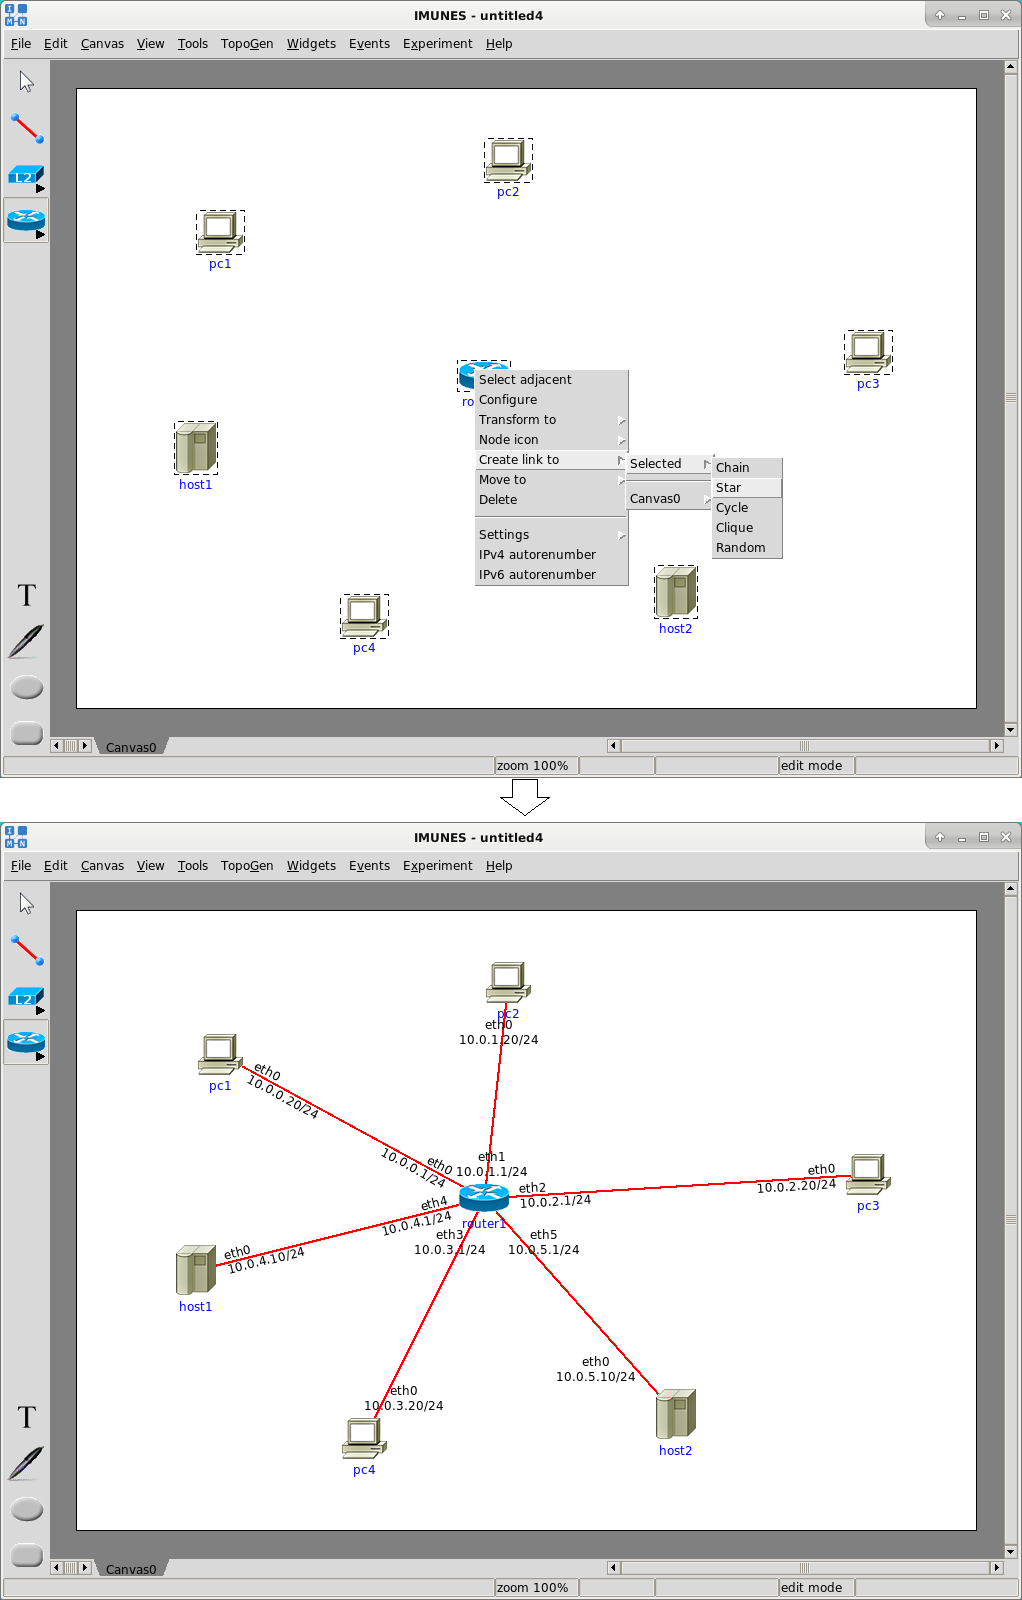
\includegraphics[width=\textwidth]{./images/connect_1connect_2.png}
\caption{\emph{Example of creating a network topology with existing nodes}}
\label{fig:connect}
\end{figure}

\begin{figure}[H]
\centering
\vspace{10pt}
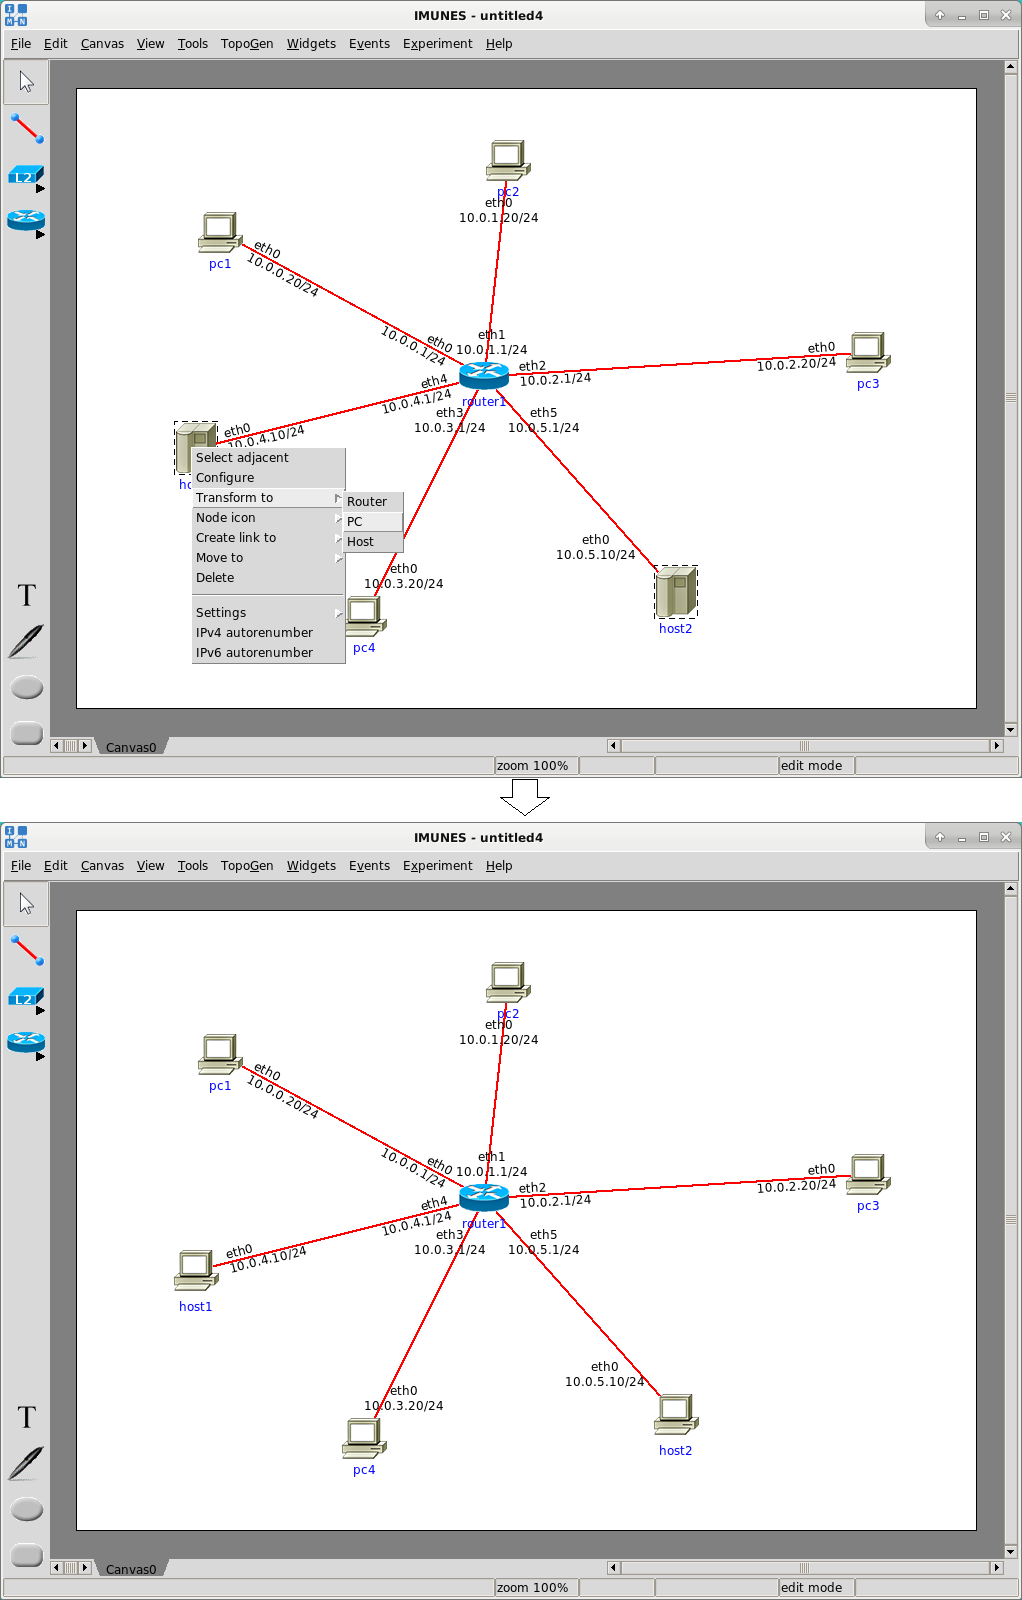
\includegraphics[width=\textwidth]{./images/transform.png}
\caption{\emph{Example of transforming existing network layer nodes}}
\label{fig:transform}
\end{figure}

\subsection{IPv4 address pool}
\label{sec:IPv4AddressPool}
\emph{IPv4 address pool} option from the \emph{Tools} menu is used for
replacing default 10.0.0.0/24 address pool. Choosing that option invokes a
dialog shown in Figure \ref{fig:ipv4_addr_pool}.

\begin{figure}[H]
\centering
\vspace{10pt}
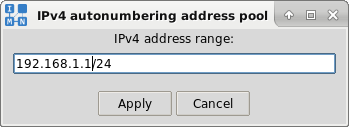
\includegraphics[width=0.35\textwidth]{./images/ipv4_addr_pool.png}
\caption{\emph{IPv4 address pool dialog}}
\label{fig:ipv4_addr_pool}
\end{figure}

In order to replace default 10.0.0.0/24 address pool, set variable-mask IPv4
address pool through the invoked dialog. CIDR notation is required, so the IPv4
address needs to be followed by a slash and a network length. To apply changes
click on the \emph{Apply} button. The given address pool will be applied to all
the subsequentially created network layer elements (Figure
\ref{fig:ipv4_addr_pool_example}).

\begin{figure}[H]
\centering
\vspace{10pt}
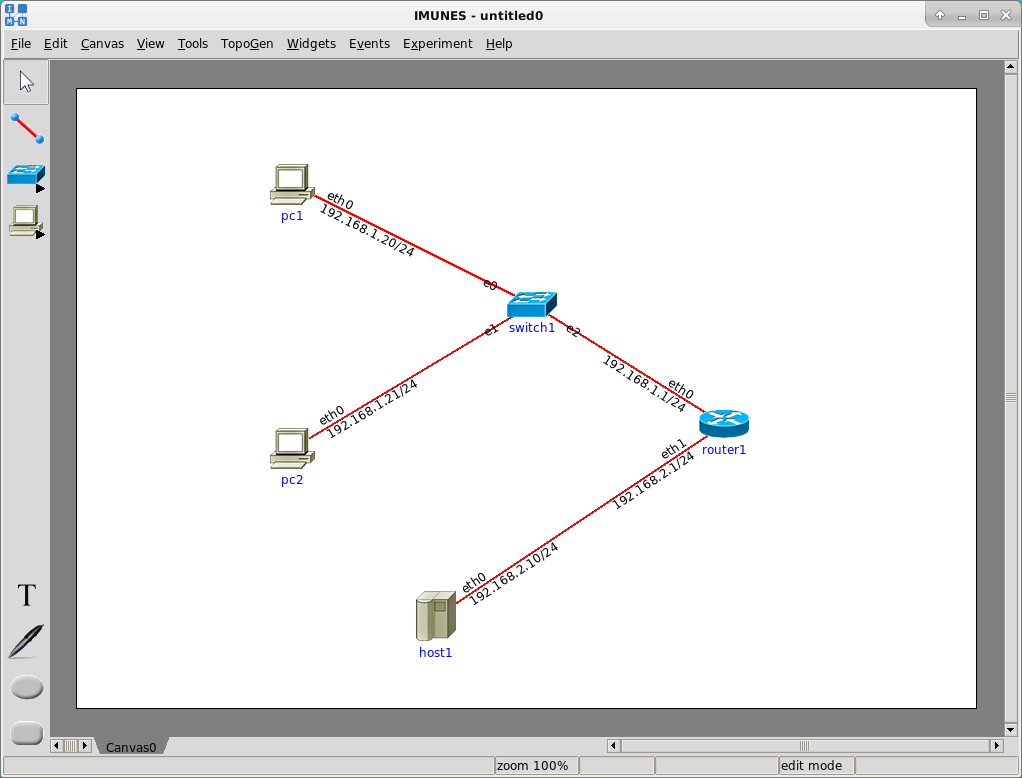
\includegraphics[width=\textwidth]{./images/ipv4_addr_pool_example.png}
\caption{\emph{IPv4 address pool example}}
\label{fig:ipv4_addr_pool_example}
\end{figure}

In order to apply the given address pool to selected elements, right click on
the network layer element and choose the option \emph{IPv4 autorenumber} from
the popped up menu. In example shown in Figure
\ref{fig:ipv4_autorenumber_example} we have set IPv4 address pool to
160.153.1.1/24, selected all network elements and selected the option
\emph{IPv4 autorenumber} from the node menu to apply the given address pool to
selected elements.

\begin{figure}[H]
\centering
\vspace{10pt}
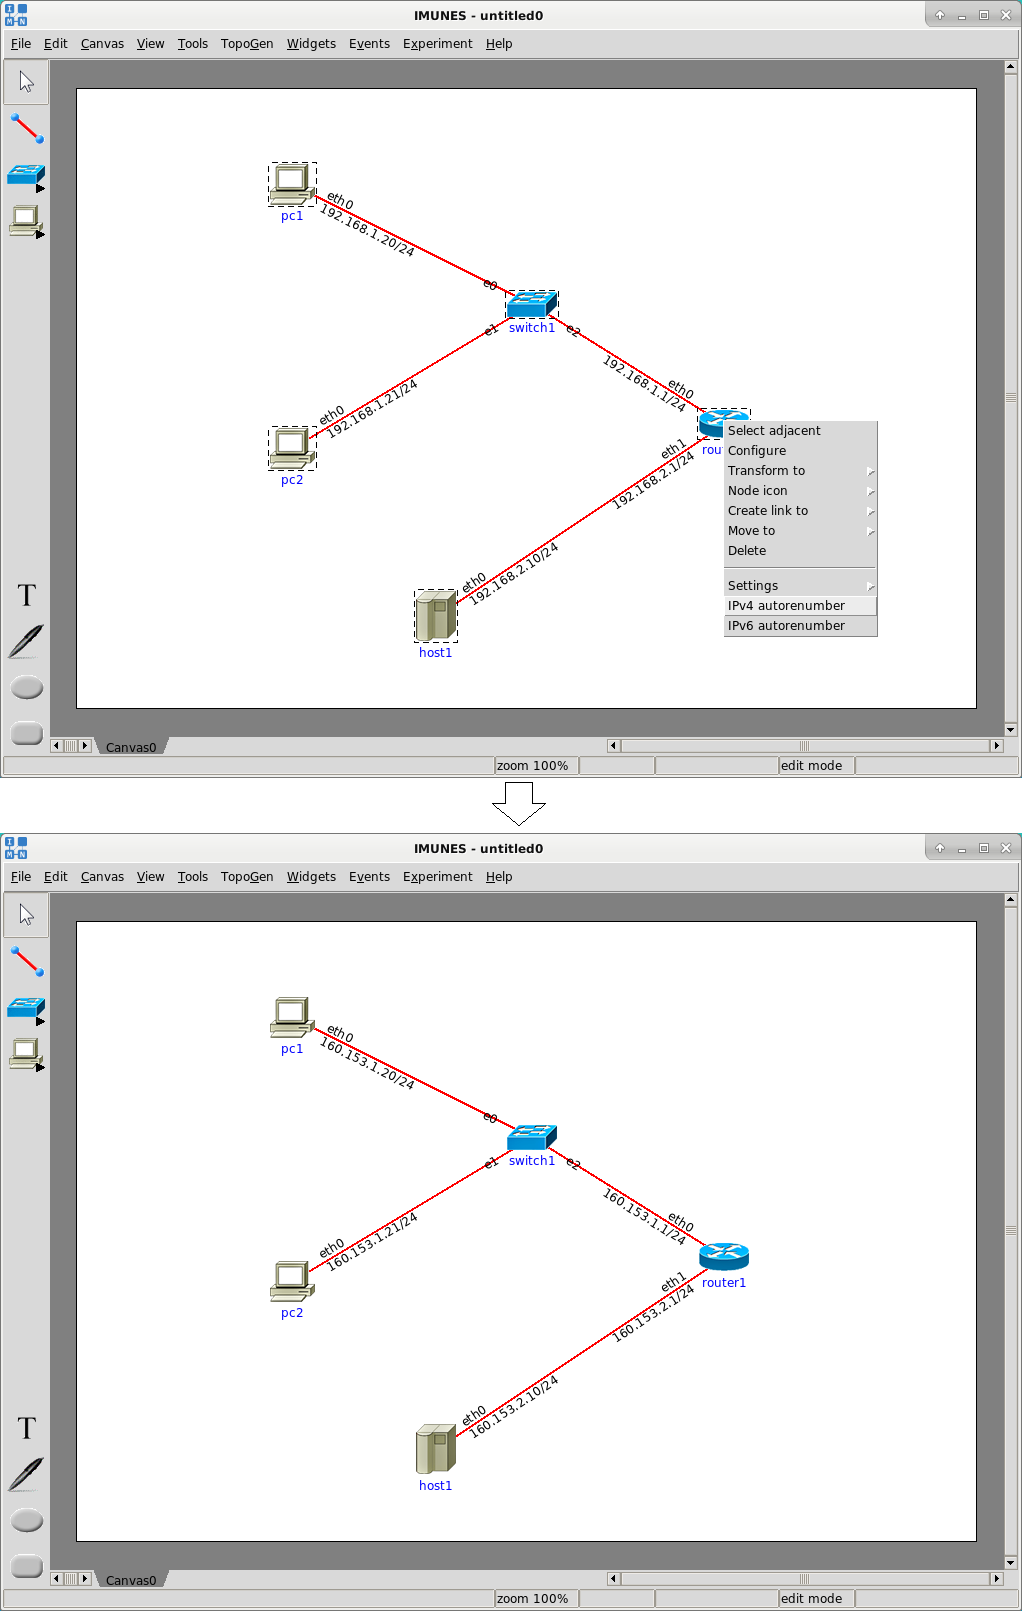
\includegraphics[width=\textwidth]{./images/ipv4_autorenumber_example.png}
\caption{\emph{IPv4 autorenumber example}}
\label{fig:ipv4_autorenumber_example}
\end{figure}

\subsection{IPv6 address pool}
\label{sec:IPv6AddressPool}
\emph{IPv6 address pool} option from the \emph{Tools} menu is used for
replacing default fc00::/64 address pool.
The procedure for setting the IPv6 address pool is the same as for setting the IPv4 address pool.

\subsection{Routing protocol defaults}
\label{sec:RoutingProtocolDefaults}
In the \emph{Tools} menu you can find the \emph{Routing protocol defaults}
option. Selecting this option invokes a popup window shown in Figure
\ref{fig:router_def_1}. Just as a reminder, settings referring to routing
protocols can be also changed in the \emph{router configuration} window. The
difference is that changes made there are applied only to the router that is
being configured. This tool in contrary makes it possible to apply changes to
one or more selected routers. If there is no router selected than the changes
will be applied to subsequentially created routers. Note that this option will
be disabled when the experiment starts.

\begin{figure}[H]
\centering
\vspace{10pt}
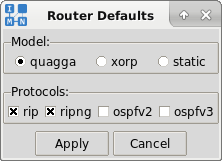
\includegraphics[width=0.35\textwidth]{./images/router_defaults_1.png}
\caption{\emph{Router defaults window}}
\label{fig:router_def_1}
\end{figure}
